\documentclass[a4paper,10pt]{report}

\usepackage{multirow}
\usepackage[english,brazil,brazilian]{babel}
\usepackage[utf8]{inputenc}
 \usepackage{graphicx}
 
\begin{document}

\section*{Cronograma}

O cronograma será seguido como descrito na Tab. \ref{fig:cronograma2} com as atividades detalhadas a seguir:

\begin{itemize}
	\item projeto protótipo 2: projeto de nova mecânica dado as necessidades levantadas no primeiro protótipo;
	\item prototipagem mecânica : envio da peça para usinagem e acompanhamento;
	\item projeto do controlador : projetar controle para estabilização do mancal visando a implementação em eletrônica embarcada;
	\item validação do protótipo : validar o protótipo com o modelo em elementos finitos (forças);
	\item projeto eletrônica : projetar eletrônica (processamento, sensoriamento e potência) com os requisitos levantados durante a pesquisa;
	\item prototipagem eletrônica : confecção e montagem de placa de circuito impresso além de compra de materiais;
	\item validação eletrônica : validar a eletrônica (programação do microprocessador, atuadores e sensores);
	\item validação do conjunto : implementação das leis de controle e teste do controle do mancal
	\item documentação : tempo reservado para a documentação e escrita da dissertação.	
\end{itemize}

\begin{figure}[th!]
\centering
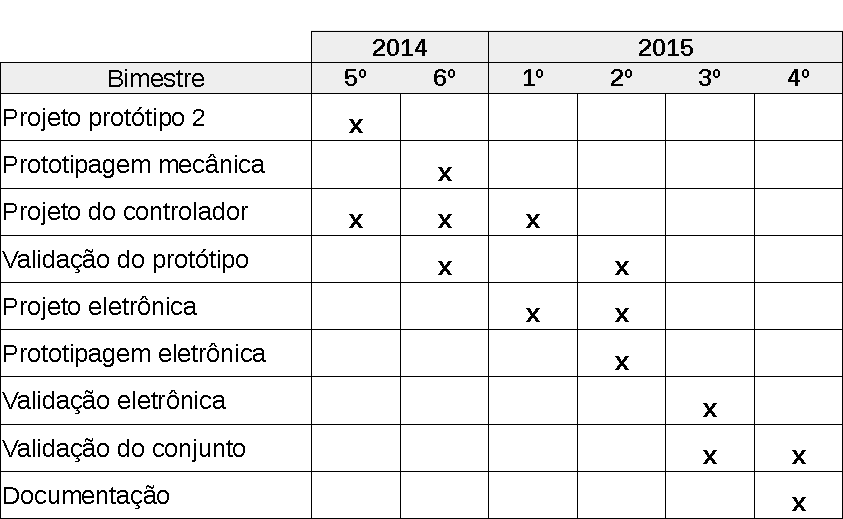
\includegraphics[width=1\linewidth]{./cronograma2}
\caption{Cronograma proposto}
\label{fig:cronograma2}
\end{figure}

\renewcommand\contentsname{Sumário Estruturado da Dissertação}
\tableofcontents


\chapter{Introdução}\label{intro}
\section{Objetivo}
\section{Justificativa}
\section{Revisão bibliográfica}
\subsection{Graus de liberdade}
\subsection{Topologias com aplicação em rodas de reação}
\subsection{Sensoriamento}
\subsection{Mancais auxiliares}
\subsection{Técnicas de controle}
\subsection{Macais magnéticos auto girantes}
\section{Metodologia}

\chapter{Mancal magnético}
\section{Visão Geral}
\section{Estator externo}\label{cap:mancal:estator:externo}
\section{Rotor}
\section{Estator interno}
\section{Batente}
\section{Base}
\section{Eletrônica}
	\subsection{Atuador - Potência}
	\subsection{Sensoreamento}
	\subsection{Processamento}
\section{Prototipagem}
\chapter{Modelagem Eletromagnética do Mancal}
\section{Circuito passivo}
\subsection{Campo magnético no entreferro}
\subsection{Força}
\subsection{Escolha dos parâmetros}
\subsection{Simulações}
\subsection{Elementos Finitos}
\subsection{Validação}

\section{Circuito Ativo}
\subsection{Modelo sem saturação}
\subsection{Indutância} \label{subsec:at:indutancia}
\section{Escolha dos parâmetros}
\subsection{Simulações}
\subsection{Elementos Finitos}
\subsection{Validação}

\chapter{Modelagem Dinâmica} \label{Cap:Modelagem:Dinamica}
\section{Rotor}
\section{Estator externo}
\section{Estator interno}
\subsection{Linearização da força}
\section{Característica do sistema e diagrama de blocos}
\section{Simulações}
\section{Validação}

\chapter{Projeto do controlador}
\section{Técnicas de controle}
\section{Simulações}
\section{Implementação}
\section{Validação}

\chapter{Conclusões}

\end{document}